\chapter{Angular Momentum and Spin}
%===========================================
\section{Eigenvalues of Angular Momentum Operators}
%===========================================

The angular momentum operator is defined as $\mathbf{L} = \mathbf{r} \times \mathbf{p}$, with components:
\[
    \hat{L}_x = y\hat{p}_z - z\hat{p}_y, \quad
    \hat{L}_y = z\hat{p}_x - x\hat{p}_z, \quad
    \hat{L}_z = x\hat{p}_y - y\hat{p}_x
\]
%
Since $x, y, z$ do not commute with $\hat{p}_x, \hat{p}_y, \hat{p}_z$ respectively, the three components of $\mathbf{L}$ do not commute with each other. However, they all commute with the total angular momentum squared operator:
\[
    \hat{L}^2 = \hat{L}_x^2 + \hat{L}_y^2 + \hat{L}_z^2
\]
%
Therefore, $\hat{L}^2$ and any one component (conventionally $\hat{L}_z$) share common eigenfunctions, see \ref{commutator}.

\subsection{Ladder Operators}

To solve for the eigenvalues, we introduce the \emph{ladder operators} due to the square-sum form of $\hat{L}_{x,y}$:

\[
    \hat{L}_x^2 + \hat{L}_y^2 = \hat{L}^2 - \hat{L}_z^2 
    \quad \Rightarrow \quad
    \hat{L}_{\pm} = \hat{L}_x \pm i\hat{L}_y
\]
%
The commutation relations are:
\[
    [\hat{L}^2, \hat{L}_{\pm}] = 0, \quad [\hat{L}_z, \hat{L}_{\pm}] = \pm\hbar\hat{L}_{\pm}, \quad \hat{L}_{\pm}\hat{L}_{\mp} = \hat{L}^2 - \hat{L}_z^2 \pm \hbar\hat{L}_z
\]
If $f$ is a simultaneous eigenfunction of $\hat{L}^2$ and $\hat{L}_z$:
\[
    \hat{L}^2 f = \lambda f, \quad \hat{L}_z f = \mu f
\]
Then applying the ladder operators:
\[\begin{aligned}
    \hat{L}^2(\hat{L}_{\pm}f) &= \hat{L}_{\pm}(\hat{L}^2f)  = \lambda(\hat{L}_{\pm}f) \\
    \hat{L}_z(\hat{L}_{\pm}f) &= [\hat{L}_z, \hat{L}_{\pm}]f + \hat{L}_{\pm}(\hat{L}_{z}f) = (\mu \pm \hbar)(\hat{L}_{\pm}f)
\end{aligned}\]\\
Thus the total angular momentum $\hat{L}^2$ is \emph{conserved} as the eigenvalue of $\hat{L}_{\pm}f$ won't change.\\
Meanwhile, $\hat{L}_{\pm}$ raises/lowers the eigenvalue of $\hat{L}_z$ by $\hbar$, so it's reasonable to assume $\mu$ as a multiple of $\hbar$ which we will employ in the next section.\\


\subsection{Quantization of Eigenvalues}

Since the $z$-component cannot exceed the total magnitude, there exist upper and lower bounds. Let:
\begin{itemize}
    \item Upper bound: $\hat{L}_+ f_{\text{t}} = 0$ with $\hat{L}_z f_{\text{t}} = \ell\hbar f_{\text{t}}$
    \item Lower bound: $\hat{L}_- f_{\text{b}} = 0$ with $\hat{L}_z f_{\text{b}} = \bar{\ell}\hbar f_{\text{b}}$
\end{itemize}
Using $\hat{L}^2 = \hat{L}_{\pm}\hat{L}_{\mp} + \hat{L}_z^2 \mp \hbar\hat{L}_z$:
\[\begin{aligned}
    \hat{L}^2 f_{\text{t}} &= \hbar^2\ell(\ell+1)f_{\text{t}} \\
    \hat{L}^2 f_{\text{b}} &= \hbar^2\bar{\ell}(\bar{\ell}-1)f_{\text{b}}
\end{aligned}\]\\
Since the total angular momentum is conserved, i.e. $\hat{L}^2$ is unchanged: $\ell(\ell+1) = \bar{\ell}(\bar{\ell}-1) \Rightarrow \bar{\ell} = -\ell$.\\
Therefore for the eigenvalue $m\hbar$ of $\hat{L}_z$, the quantum number $m$ takes values from $-\ell$ to $+\ell$ in integer steps. If $N$ steps are needed:
\[
    \ell = -\ell + N \quad \Rightarrow \quad \ell = \frac{N}{2}
\]
Which implies that $\ell$ is either an integer or a half integer:
\[
    \boxed{\ell = 0, \frac{1}{2}, 1, \frac{3}{2}, \ldots; \quad m = -\ell, -\ell+1, \ldots, \ell-1, \ell}
\]\\
Thus an angular momentum state depends on two quantum numbers $\ell$ and $m$ in accordance to:
\[
\hat{L}^2\ket{\ell, m} = \hbar^2\ell(\ell+1)\ket{\ell, m}, \quad
\hat{L}_z\ket{\ell, m} = \hbar m\ket{\ell, m}
\]
\emph{Physical interpretation}: For a fixed angular momentum magnitude, the vector lies on a sphere. The $z$-component takes discrete values, meaning the angular momentum vector precesses around the $z$-axis on cones.

%===========================================
\section{Eigenfunctions of Angular Momentum}
%===========================================

In spherical coordinates $(r, \theta, \varphi)$:
\[
    \mathbf{L} = -i\hbar\left(\hat{\varphi}\pdv{\theta} - \hat{\theta}\frac{1}{\sin\theta}\pdv{\varphi}\right)
\]\\
The squared operator becomes:
\[
    \hat{L}^2 = -\hbar^2\left[\frac{1}{\sin\theta}\pdv{\theta}\left(\sin\theta\pdv{\theta}\right) + \frac{1}{\sin^2\theta}\pdv[2]{\varphi}\right]
\]\\
The eigenfunctions are the \emph{spherical harmonics}:
\[
    \hat{L}^2 Y_{\ell}^{m}(\theta,\varphi) = \hbar^2\ell(\ell+1)Y_{\ell}^{m}(\theta,\varphi)
\]\\
For the $z$-component:
\[
    \hat{L}_z = -i\hbar\pdv{\varphi} \quad \Rightarrow \quad f_\varphi = \frac{1}{\sqrt{2\pi}}e^{im\varphi}
\]\\
This is part of the spherical harmonic. Note that for orbital angular momentum, $\ell$ must be an integer due to the requirement of spherical harmonics.

%===========================================
\section{Spin and Spin Operators}\label{spin1}
%===========================================

Elementary particles possess intrinsic angular momentum (\emph{spin}) $\mathbf{S}$ even without spatial rotation, manifesting in properties like magnetic moments.\\ \\
Spin operators follow the same algebra as orbital angular momentum:
\[
    [\hat{S}_x, \hat{S}_y] = i\hbar\hat{S}_z, \quad
    [\hat{S}_y, \hat{S}_z] = i\hbar\hat{S}_x, \quad
    [\hat{S}_z, \hat{S}_x] = i\hbar\hat{S}_y
\]
Acting on quantum states:
\[\begin{aligned}
    \hat{S}^2\ket{s,m} &= \hbar^2 s(s+1)\ket{s,m} \\
    \hat{S}_z\ket{s,m} &= \hbar m\ket{s,m} \\
    \hat{S}_{\pm}\ket{s,m} &= \hbar\sqrt{s(s+1)-m(m\pm1)}\ket{s,m\pm1}
\end{aligned}\]

\subsection{Spin-1/2 and Pauli Matrices}

For $s = 1/2$, we have $m = \pm1/2$. Define the basis states:
\[
    \ket{\uparrow} = \ket{\tfrac{1}{2},\tfrac{1}{2}} = \begin{pmatrix} 1 \\ 0 \end{pmatrix}, \quad
    \ket{\downarrow} = \ket{\tfrac{1}{2},-\tfrac{1}{2}} = \begin{pmatrix} 0 \\ 1 \end{pmatrix}
\]\\
A general spin state can be expressed as a \emph{spinor} with 
$\chi_+ = \ketup$ and $\chi_-=\ketdown$:

\[
    \chi = \begin{pmatrix} a \\ b \end{pmatrix} = a\chi_+ + b\chi_-, \quad |a|^2 + |b|^2 = 1
\]
The spin operators then comes in matrix form according to eigenvalue equation:
\[\begin{aligned}
    \hat{S}^2 &= \frac{3}{4}\hbar^2\begin{pmatrix} 1 & 0 \\ 0 & 1 \end{pmatrix}, &
    \hat{S}_z &= \frac{\hbar}{2}\begin{pmatrix} 1 & 0 \\ 0 & -1 \end{pmatrix} \\
    \hat{S}_+ &= \hbar\begin{pmatrix} 0 & 1 \\ 0 & 0 \end{pmatrix}, &
    \hat{S}_- &= \hbar\begin{pmatrix} 0 & 0 \\ 1 & 0 \end{pmatrix} \\
    \hat{S}_x &= \frac{\hbar}{2}\begin{pmatrix} 0 & 1 \\ 1 & 0 \end{pmatrix}, &
    \hat{S}_y &= \frac{\hbar}{2}\begin{pmatrix} 0 & -i \\ i & 0 \end{pmatrix}
\end{aligned}\]\\
Removing the factor $\hbar/2$, we obtain the \emph{Pauli matrices}:
\[
    \sigma_x = \begin{pmatrix} 0 & 1 \\ 1 & 0 \end{pmatrix}, \quad
    \sigma_y = \begin{pmatrix} 0 & -i \\ i & 0 \end{pmatrix}, \quad
    \sigma_z = \begin{pmatrix} 1 & 0 \\ 0 & -1 \end{pmatrix}
\]\\
Eigenstates of $\hat{S}_x$:
\[
    \chi_{\pm}^{(x)} = \frac{1}{\sqrt{2}}\begin{pmatrix} 1 \\ \pm 1 \end{pmatrix}, \quad \text{eigenvalues } \pm\frac{\hbar}{2}
\]\\
Any state can then also be expressed in the eigenstates of $\hat{S}_x$:
\[
    \chi = \left(\frac{a+b}{\sqrt{2}}\right)\chi_+^{(x)} + \left(\frac{a-b}{\sqrt{2}}\right)\chi_-^{(x)}
\]

\subsection{Larmor Precession: Application of Spin}

An electron with spin has a magnetic moment $\mathbf{\mu} = \gamma\mathbf{S}$ (where $\gamma$ is the gyromagnetic ratio, see \ref{gyro}). In a magnetic field $\mathbf{B}$, the Hamiltonian is:
\[
    \hat{H} = -\mathbf{\mu}\cdot\mathbf{B}
\]\\
For a static field $\mathbf{B} = B_0\hat{k}$:
\[
    \hat{H} = -\gamma B_0 \hat{S}_z = -\frac{1}{2}\gamma B_0\hbar\begin{pmatrix} 1 & 0 \\ 0 & -1 \end{pmatrix}
\]\\
The time evolution follows the Schrödinger equation $i\hbar\partial\chi/\partial t = \hat{H}\chi$. The solution is a linear combination of eigenstates:
\[
    \chi(t) = \begin{pmatrix} a e^{i\gamma B_0 t/2} \\ b e^{-i\gamma B_0 t/2} \end{pmatrix}, \quad |a|^2 + |b|^2 = 1
\]\\
Setting $a = \cos\alpha$, $b = \sin\alpha$, the expectation values are:
\[\begin{aligned}
    \expect{\hat{S}_x} &= \frac{\hbar}{2}\sin(2\alpha)\cos(\gamma B_0 t) \\
    \expect{\hat{S}_y} &= \frac{\hbar}{2}\sin(2\alpha)\sin(\gamma B_0 t) \\
    \expect{\hat{S}_z} &= \frac{\hbar}{2}\cos(2\alpha)
\end{aligned}\]\\
\emph{Conclusion}: The spin vector $\expect{\mathbf{S}}$ precesses around the magnetic field direction at frequency $\omega = \gamma B_0$ (Larmor frequency), maintaining constant tilt angle $2\alpha$.

%===========================================
\section{Addition of Angular Momentum}
%===========================================
\subsection{Clebsch-Gordan Coefficients}
This applies not only to spin addition $\mathbf{S} = \mathbf{S}_1 + \mathbf{S}_2$, but also to $\mathbf{L}$, $\mathbf{S}$ and $\mathbf{J} = \mathbf{L} + \mathbf{S}$.\\ \\
For two particles with states $\ket{s_1,m_1}$ and $\ket{s_2,m_2}$, the composite state is $\ket{s_1,m_1}\otimes\ket{s_2,m_2}$. Since $\hat{S}_z = \hat{S}_{1z} + \hat{S}_{2z}$, we have $m = m_1 + m_2$.\\
While the $z$-components add as scalars, the total angular momentum vectors add vectorially. The possible values of total spin $s$ range from $|s_1-s_2|$ to $s_1+s_2$ in integer steps:
\[
    s = |s_1-s_2|, |s_1-s_2|+1, \ldots, s_1+s_2
\]
The product states can be decomposed into linear combinations of total angular momentum states $\ket{s,m}$ using \emph{Clebsch-Gordan coefficients}:
\[
    \ket{s_1,m_1}\otimes\ket{s_2,m_2} = \sum_{s} C_{m_1m_2m}^{s_1s_2s}\ket{s,m}, \quad (m = m_1 + m_2)
\]
Conversely:
\[
    \ket{s,m} = \sum_{m_1+m_2=m} C_{m_1m_2m}^{s_1s_2s}\ket{s_1,m_1}\otimes\ket{s_2,m_2}
\]
This process is in fact the direct sum decomposition of a direct product of two vectors, 
which will be discussed in another prespective in \ref{direct sum} and \ref{molecular term}.


\subsection{Spin-1/2 and Entanglement}
\begin{figure}
\centering
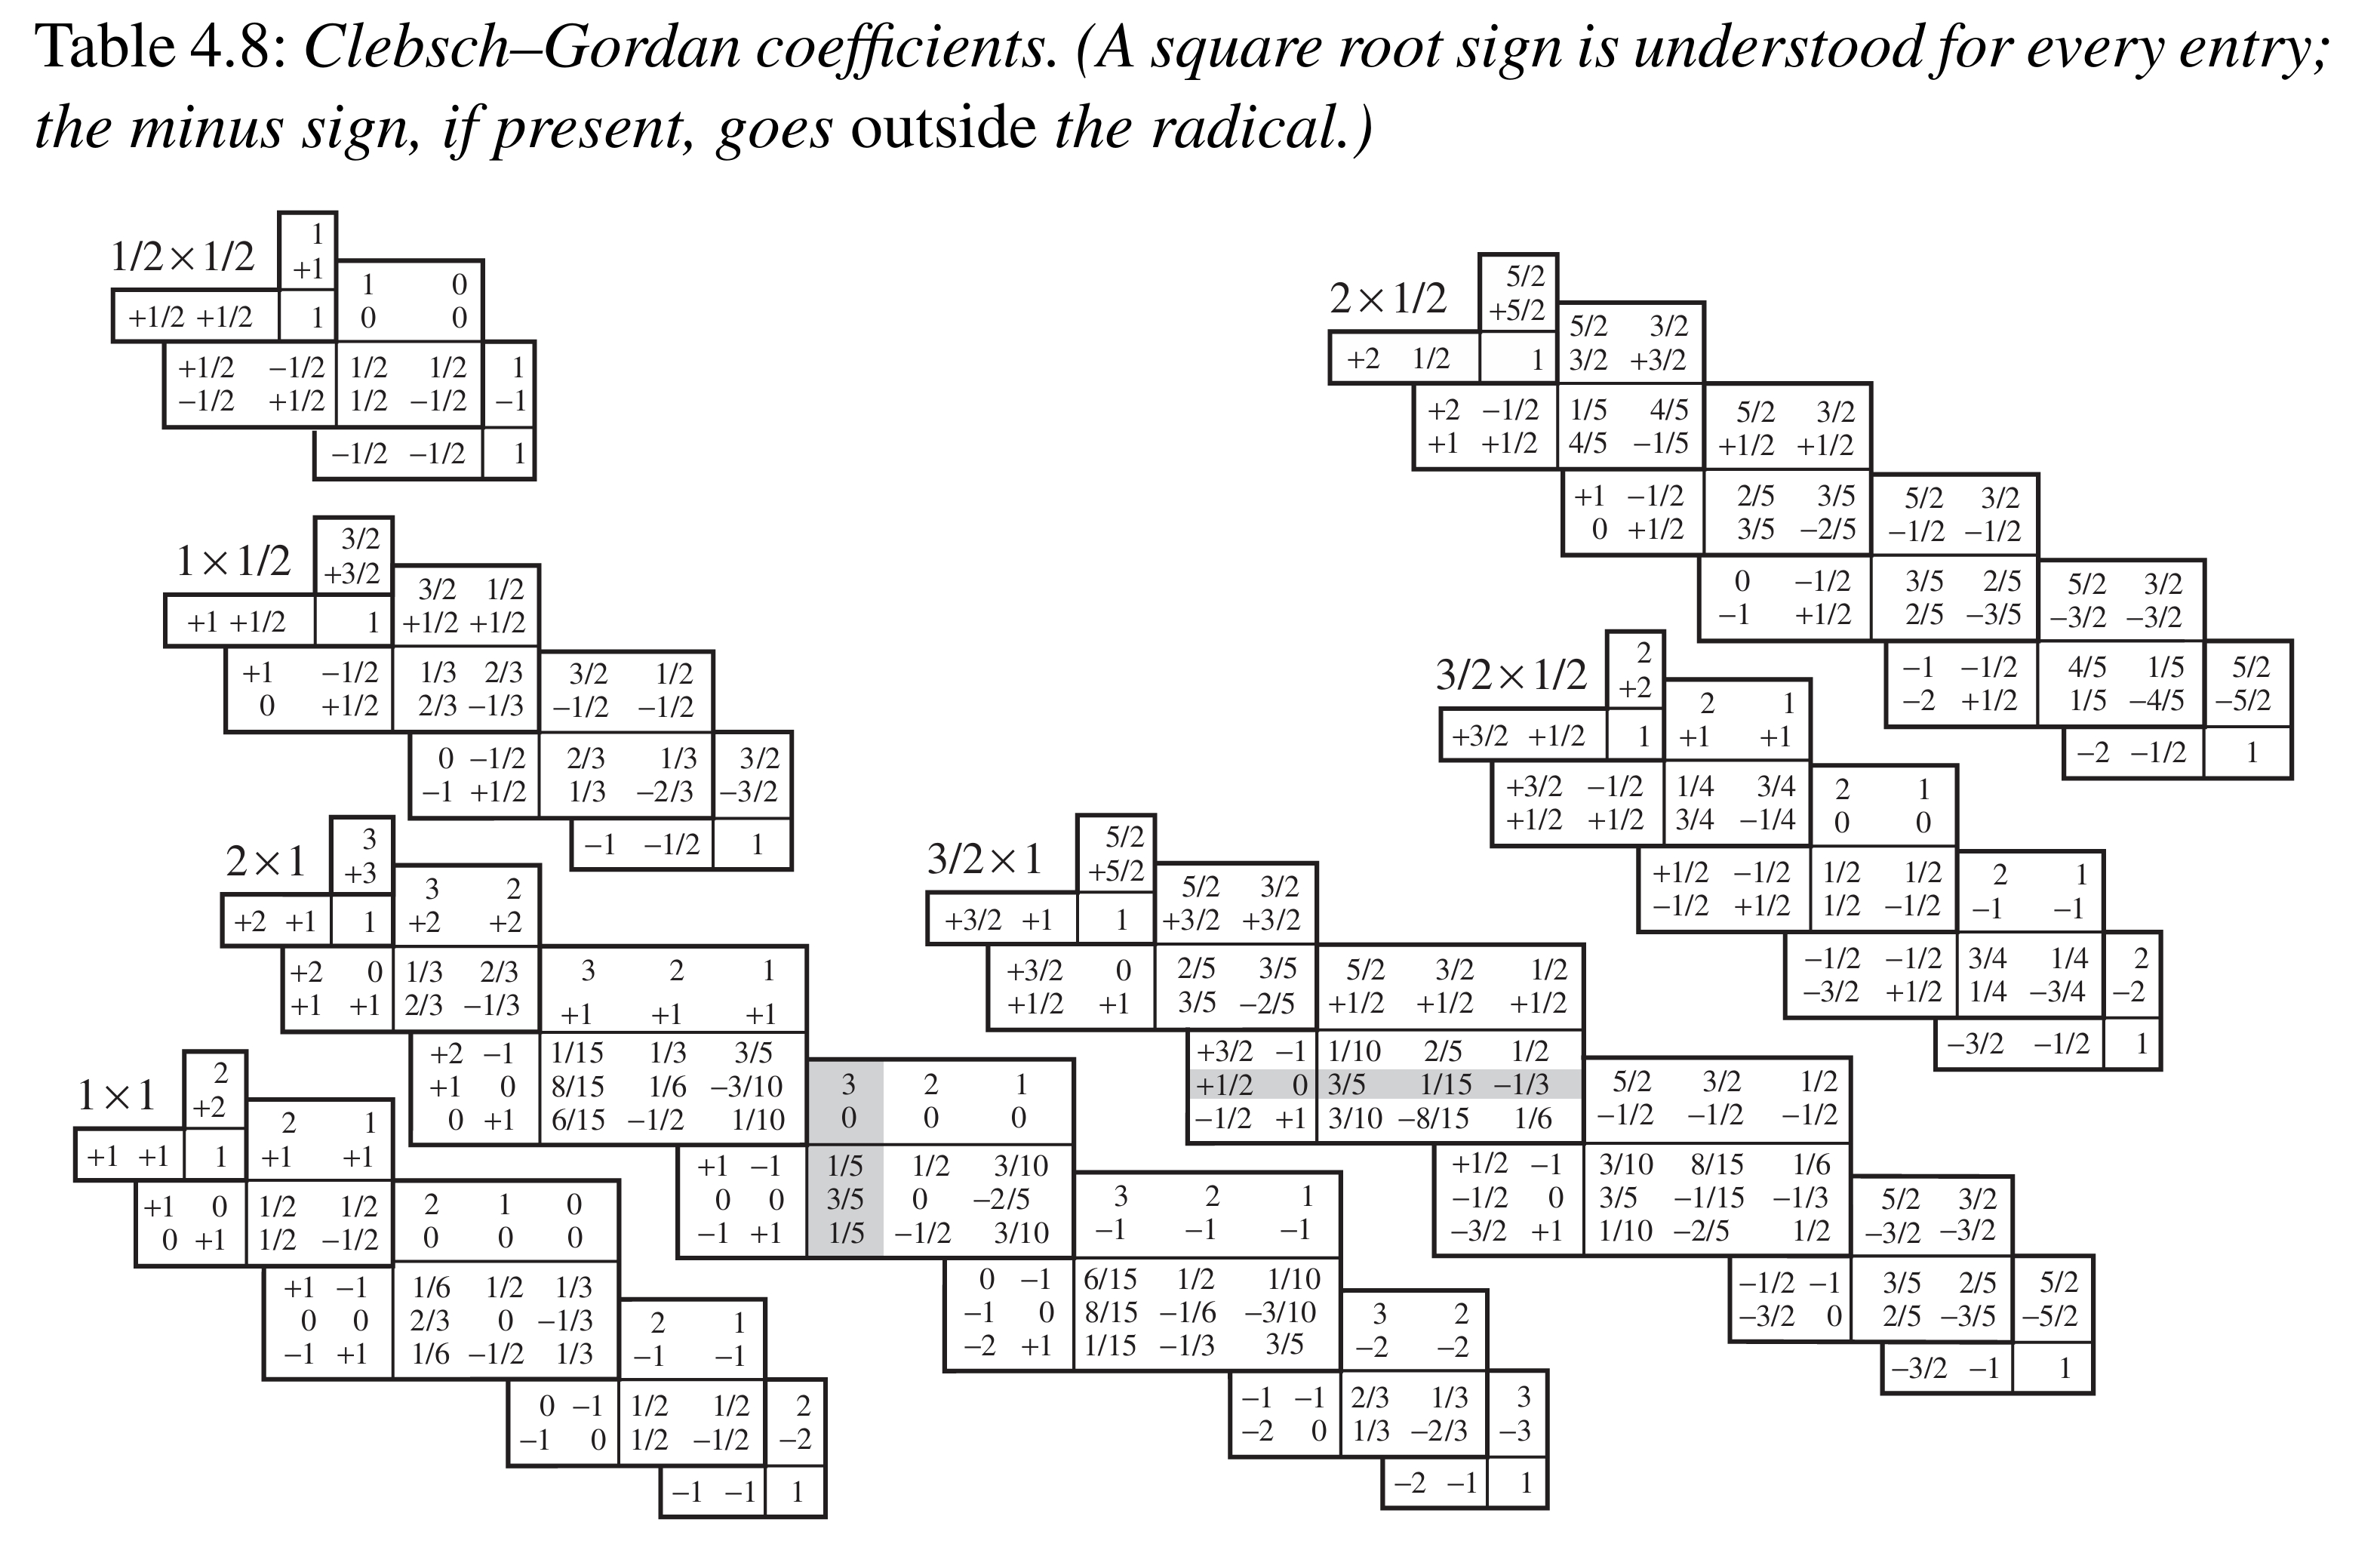
\includegraphics[scale=0.15]{Ch3/CG}
\end{figure}

For two electrons ($s_1 = s_2 = 1/2$), the CG coefficients yield:\\
\emph{Triplet states} ($s=1$, symmetric):
\[
    \ket{1,1} = \ket{\uparrow\uparrow} \quad
    \ket{1,0} = \frac{1}{\sqrt{2}}(\ket{\uparrow\downarrow} + \ket{\downarrow\uparrow}) \quad
    \ket{1,-1} = \ket{\downarrow\downarrow}
\]
\emph{Singlet state} ($s=0$, antisymmetric):
\[
    \ket{0,0} = \frac{1}{\sqrt{2}}(\ket{\uparrow\downarrow} - \ket{\downarrow\uparrow})
\]
Upon taking a further look at the singlet state, we find it in fact a superposition of two states with the same probability: 
$\ket{\uparrow_A\downarrow_B}$ and $\ket{\downarrow_A\uparrow_B}$.\\
\ If we have two electrons paired to be singlet, and $S_z$ of one electron measures +1/2 (with a probability of 50\%), 
then the state immediately collapse into either $\ket{\uparrow_A\downarrow_B}$ or $\ket{\downarrow_A\uparrow_B}$, 
depending on whether you name this electron $A$ or $B$, as electrons are identical and thus indistinguishable.\\
\ But whatever we name this electron, the other one \emph{must} have a determined opposite spin of -1/2 assigned to it 
immediately the spin of the former measures +1/2, 
which doesn't follow the probability distribution anymore, no matter how far they are separated and how many times you measure it.\\ \\
This spooky action at a distance in which the state of a particle is directly determined by another is called \emph{entanglement}, 
which proves real in \emph{Bell's inequality experiment}.
We will encounter this phenomenon again in \ref{entangle} when we talk about identical particles.\label{entangle2}



